\documentclass[a4paper,12pt]{report}
%\documentclass[a4paper,10pt]{scrartcl}

\usepackage[utf8]{inputenc}
\usepackage[T1]{fontenc}
\usepackage{graphicx}
% \usepackage{hyperref}
\usepackage{tikz}
\usepackage[margin=0.75in]{geometry}
\usetikzlibrary{arrows}

\renewcommand{\contentsname}{Sommaire}

\renewcommand{\chaptername}{}
\setcounter{chapter}{-1}

\tikzset{
  treenode/.style = {align=center, inner sep=0pt, text centered,
    font=\sffamily},
  arn_n/.style = {treenode, circle, draw=black, text width=2em},
  arn_x/.style = {treenode, rectangle, draw=black, text width=1.5em,
    minimum width=1.5em, minimum height=1.5em}
}

\title{\Huge Rapport \\ Projet ALGAV Trie \\ \large Implantation du Trie Hybride et du Patricia Trie}
\author{Amel ARKOUB 3301571 \\ Ling-Chun SO 3414546}
\date{22 décembre 2017}

\pdfinfo{%
  /Title    ()
  /Author   ()
  /Creator  ()
  /Producer ()
  /Subject  ()
  /Keywords ()
}

\begin{document}
\maketitle

\tableofcontents
\newpage

\chapter{Introduction}
\section*{Présentation}
\paragraph*{}
Nous souhaitons représenter un dictionnaire de mots, c'est-à-dire implanter une structure de
données efficace stockant des mots. Pour cela, nous allons nous servir de la structure de {\itshape trie}.
Dans cette optique, nous proposons les implantations de deux structures de tries concurrentes : le trie hybride
et le PATRICIA trie. Ensuite, nous effectuerons une étude expérimentale dans laquelle nous analyserons les résultats, afin de mettre en exergue
les avantages et inconvénients de chacune des structures. Nous avons choisi le langage de programmation Java pour nos implantations.

\section*{Trie}
Un trie est une représentation arborescente d'un ensemble de clés qui permet d'éviter la répétition de préfixes communs des mots.

\section*{Trie Hybride}
Un trie hybride est un arbre ternaire dont chaque nœud contient un caractère et une valeur (non vide
lorsque le nœud représente une clé). Chaque nœud a 3 pointeurs: un lien Inf (resp. Eq, res. Sup) vers le sous-arbre dont le premier caractère est inférieur (resp. égal, resp. supérieur) à son caractère. Il permet en outre
de réduire le nombre de pointeurs vides par rapport à un R-Trie.

\section*{PATRICIA Trie}
Un PATRICIA trie est un arbre dont le but est de réduire la hauteur des R-Trie tout en conservant une recherche
efficace. Pour ce faire, plutôt que chaque nœud interne ait pour valeur une lettre, il a pour valeur le préfixe commun à un ensemble de mots.

\chapter{Trie Hybride}
\section{Implantation}
Dans notre implantation JAVA, un trie hybride est un objet qui contient 5 éléments:
\begin{itemize}
 \item un char ``letter'', qui correspond à la lettre stockée.
 \item une valeur ``value'', qui correspond à la représentation de fin de mot (-1 le nœud n'est pas la fin
 d'un mot, sinon la valeur correspond à l'ordre d'ajout croissant).
 \item un pointeur vers un trie hybride ``fc'', ce trie hybride correspond au fils central, c'est-à-dire on parcours ce
 trie hybride si le caractère recherché au Trie Hybride courant est correct.
 \item un pointeur vers un trie hybride ``fg'', ce trie hybride correspond au fils gauche, c'est-à-dire on parcours ce
 trie hybride si le caractère recherché au Trie Hybride courant est plus petit dans l'ordre alphabétique.
 \item un pointeur vers un trie hybride ``fd'', ce trie hybride correspond au fils droit, c'est-à-dire on parcourt ce
 trie hybride si le caractère recherché au trie hybride courant est plus grand dans l'ordre alphabétique.
\end{itemize}

\paragraph*{}
Voici une représentation du trie hybride résultant des ajouts successifs des mots:
\begin{itemize}
 \item don
 \item le
 \item a
 \item dort
\end{itemize}

\begin{center}
\begin{tikzpicture}[->,>=stealth',level/.style={sibling distance = 6cm/#1,
  level distance = 2.5cm}]
\node [arn_n] {d \\ -1}
    child{ node [arn_n] {a \\ 2}}
    child{ node [arn_n] {o \\ -1}
	    child{ node [arn_x] {}}
            child{ node [arn_n] {n \\ 0} 
							child{ node [arn_x] {}}
							child{ node [arn_x] {}}
							child{ node [arn_n] {r \\ -1}
							      child{ node [arn_n] {t \\ 3}}
							}	
            }
            child{ node [arn_x] {}}
		}
    child{ node [arn_n] {l \\ -1}
	    child{ node [arn_n] {e \\ 1}}
    }
; 
\end{tikzpicture}
\end{center}

\begin{figure}[!htbp]
\caption{Représentation d'un Trie Hybride}
\end{figure}

\section{Description des algorithmes}
\subsection{Algorithmes triviaux}
La plupart des algorithmes de l'implantation du trie hybride sont relativement triviaux, notamment
les fonctions:
\begin{itemize}
 \item Recherche(arbre, mot) $\rightarrow$ booléen
 \item ComptageMots(arbre) $\rightarrow$ entier
 \item ListeMots(arbre) $\rightarrow$ liste[mots]
 \item ComptageNil(arbre) $\rightarrow$ entier
 \item Hauteur(arbre) $\rightarrow$ entier
 \item ProfondeurMoyenne(arbre) $\rightarrow$ entier
 \item Prefixe(arbre) $\rightarrow$ entier
\end{itemize}
Elles correspondent pour la plupart d'un simple parcours de la structure du trie hybride, dont le traitement
dépend de la fonction.

\subsection{AjoutMot}
La fonction ajoutMot permet d'ajouter un mot dans le trie hybride, et par conséquent la construction même du trie hybride,
dont la signature est: ajoutMot(mot, arbre) $\rightarrow$ void.
Les étapes sont donc:
\begin{itemize}
 \item le cas d'arrêt est lorsque le mot a été ajouté.
 \item si nous sommes dans la racine qui est encore vide alors on ajoute le mot (on génère la suite de noeud formant un mot).
 \item si le mot est de longueur 1, alors on vérifie si le trie hybride courant correspond à la bonne lettre
 sinon on effectue des appels récursifs sur le fils gauche ou droit.
 \item dans le cas général, on compare le caractère du mot et le caractère du trie hybride courant, si les lettres
 concordent alors on appelle récursivement sur le fils central ; si elles sont différentes, on effectue un appel récursif sur le
 fils gauche ou droit suivant l'ordre alphabétique des caractères.
\end{itemize}

\subsection{Suppression}
La fonction suppressionMot permet la suppression d'un mot dans le trie hybride et maintient le trie hybride cohérent en supprimant
les nœuds dont il n'existe pas de mot, la signature est: suppression(arbre, mot) $\rightarrow$ void.
Les étapes sont donc:
\begin{itemize}
 \item si le trie hybride courant est un pointeur null alors on a un cas d'arrêt.
 \item si le mot est réduit à une lettre alors on vérifie que le caractère du mot et du trie hybride courant sont égaux. Dans ce cas, on ne considère plus le trie hybride comme un mot. Dans le cas contraire, c'est-à-dire s'ils ne sont
 pas égaux, alors on fait un appel récursif sur le fils gauche ou droit suivant la comparaison de l'ordre alphabétique des lettres.
 \item dans le cas général, on compare le caractère du mot et le caractère du Trie Hybride courant, si les lettres
 concordent alors on appelle récursivement sur le fils central ; si elles sont différentes, on fait un appel récursif sur le
 fils gauche ou droit suivant l'ordre alphabétique des caractères.
 \item on effectue un vérification d'éxistence de mots dans les fils du trie hybride, si un fils ne possède pas de noeud mot
 alors il n'est plus référencé par le trie hybride courant.
\end{itemize}


\section{Complexité}
\subsection{Recherche}
Pour la recherche d'un mot de \textit{L} caractères et un trie hybride de taille \textit{n}, 
en prenant la comparaison de caractère comme mesure, on obtient une complexité dans le cas général en $\Theta$(L), si \textit{L} < \textit{n}
puisqu'il faut parcourir chaque caractère du mot au minimum. Sinon le pire cas est atteint en $\Theta$(n) lorsqu'il y a des
ajouts par ordre alphabétique et que le mot recherché contient une succession de lettre 'z'.

\subsection{Comptage Mots}
Le comptage de mots revient à faire un parcours de l'arbre en entier.
Soit un arbre de taille \textit{n}, en prenant la comparaison de la valeur du nœud comme mesure,
on a donc une complexité $\Theta$(n).

\subsection{Liste Mots}
La récupération des mots dans un trie hybride correspond aussi à un parcours de l'arbre en entier en gardant le \textit{préfixe}
en argument dans les appels de fonctions (il est nécessaire d'effectuer une comparaison de la \textit{valeur} de chaque noeud du
trie hybride).
Soit un arbre de taille \textit{n}, en prenant la comparaison de la valeur du nœud comme mesure,
on a donc une complexité en $\Theta$(n).

\subsection{Comptage Nil}
Le comptage de pointeur vers null correspond à un parcours de tous les nœuds afin de compter le nombre de fils null.
Soit un arbre de taille \textit{n}, en prenant la comparaison de la valeur du nœud comme mesure,
on a une complexité en $\Theta$(n) puisque pour \textit{n} noeuds, on a un nombre de comparaisons $\le$ \textit{3n}.

\subsection{Hauteur}
La détermination de la hauteur du trie hybride est un parcours complet de l'arbre, en prenant l'existence de fils comme mesure, on obtient une complexité en $\Theta$(n).

\subsection{Profondeur Moyenne}
La profondeur moyenne d'un trie hybride est un parcours jusqu'aux feuilles où on ajoute la profondeur dans une liste dont on 
effectue une division à la fin du parcours. En prenant la comparaison d'existence de fils comme mesure, on obtient une complexité
de $\Theta$(n).

\subsection{Préfixe}
La recherche du préfixe peut être dans le pire cas en $\Theta$(n). En effet, le pire cas est atteint lorsque le trie hybride
est une ``liste chaînée'' et donc à hauteur \textit{h}=n.

\subsection{Suppression}
La suppression d'un mot est une recherche dans le trie hybride, ce qui correspond à une complexité en $\Theta$(n) comparaisons
dans le pire cas. Cependant, il y a aussi 3 appels une fonction qui recherche l'existence d'un noeud mot de compléxité $\Theta$(n).
On a donc une complexité en $\mathcal{O}$($n^2$).

\chapter{PATRICIA Trie}
\section{Implantation}
Dans notre implantation JAVA, un PATRICIA trie est représenté par :
\begin{itemize}
\item une chaîne de caractères, nommée {\itshape valeur}, qui est le préfixe.
\item un tableau de 27 PATRICIA tries fils {\itshape patTries}, un pour chaque lettre de l'alphabet, le 27ème représentant le caractère de fin de mot. Ce caractère est "\{" .
\item un indice, entier nommé {\itshape ind}, qui est le numéro de la prochaine lettre à évaluer dans les mots fils. En effet, les mots fils ont ce même préfixe, et diffèrent à partir de la lettre indiquée par l'indice.
\item un booléen, {\itshape isFeuille} indiquant si ce nœud est une feuille ou non. Dans le cas où le nœud est une feuille, le préfixe est en fait le mot en entier.
\end{itemize}
 \bigbreak

Voici un exemple de la structure de données après les insertions des mots "saler", "sale" et "salut".

\begin{center}
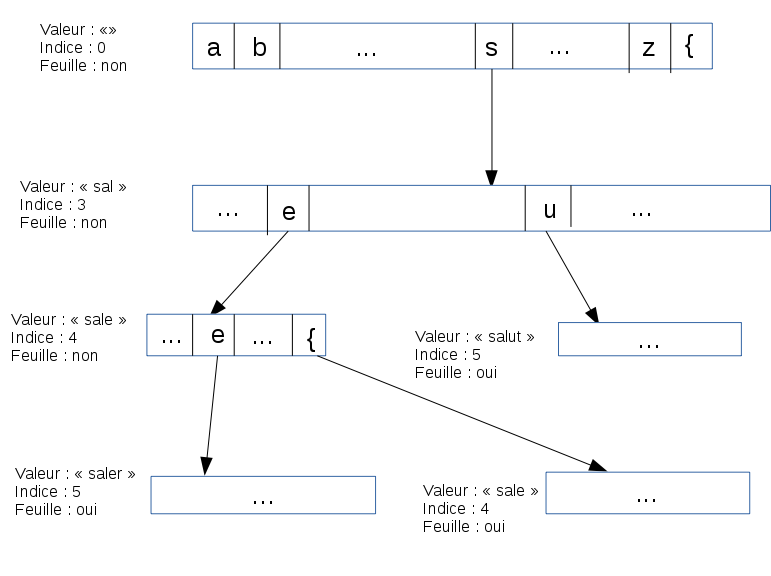
\includegraphics[scale=0.40]{../rapport/Schema_PAT_trie.png}
\end{center}
\begin{figure}
\caption{Représentation graphique d'un PATRICIA trie}
\end{figure}



\section{Description des algorithmes}
\subsection{Algorithmes triviaux}
Voici les algorithmes triviaux, qui correspondent essentiellement à un simple parcours du PATRICIA trie, et qui ne nécessitent pas une explication appronfondie :
\begin{itemize}
 \item Recherche(PATRICIA trie, mot) $\rightarrow$ booléen
 \item ComptageMots(PATRICIA trie) $\rightarrow$ entier
 \item ListeMots(PATRICIA trie) $\rightarrow$ liste[mots]
 \item ComptageNil(PATRICIA trie) $\rightarrow$ entier
 \item Hauteur(PATRICIA trie) $\rightarrow$ entier
 \item ProfondeurMoyenne(PATRICIA trie) $\rightarrow$ flottant
 \item Prefixe(PATRICIA trie) $\rightarrow$ entier
\end{itemize}

\subsection{Ajouter un mot}
La fonction ajouterMot permet d'ajouter un mot qui n'est pas déjà présent dans le PATRICIA trie. La signature est: ajouterMot(PATRICIA trie, mot) $\rightarrow$ booléen.
Voici une description succincte de l'algorithme :

Si la taille du mot à ajouter équivaut à celle du préfixe du PATRICIA trie :
\begin{itemize}
	\item s'il existe déjà un PATRICIA trie fils de fin de mot, c'est-à-dire celui qui se trouve à la case correspondant au caractère de fin de mot "\{", on renvoie FAUX. En effet, cela signifie qu'il est déjà présent. 
	\item sinon, on le crée puis on renvoie VRAI.
\end{itemize}
\smallbreak
Sinon on regarde le PATRICIA trie fils se trouvant à la lettre indiquée par l'indice du PATRICIA trie courant.
\begin{itemize}
	\item si la case indiquée est un pointeur vers NIL, alors on crée à cette case un nouveau PATRICIA trie, ayant pour valeur le mot, pour indice l'indice du père + 1 et est considéré comme une feuille. Ensuite, on renvoie VRAI.
	\item sinon un PATRICIA trie fils existe déjà à cette case, et alors il faut comparer sa valeur avec le mot qu'on veut ajouter.
	\begin{itemize}
			\item si sa valeur, notée val, est correspond au préfixe du mot à ajouter, alors on fait un appel récursif sur ce PATRICIA trie.
			\item sinon, on compare val avec le mot à ajouter, pour trouver l'indice à partir duquel ils diffèrent. En effet, on doit créer un PATRICIA trie qui contient le préfixe commun de val et du mot à ajouter, puis créer des PATRICIA tries fils à ce nouveau PATRICIA trie, qui contiendront val et le mot à ajouter.
	\end{itemize}
	Finalement, on renvoie VRAI.
\end{itemize}


\subsection{Supprimer un mot}
La fonction supprimerMot permet la suppression d'un mot dans le PATRICIA trie et maintient ce PATRICIA trie cohérent en supprimant
les nœuds dont il n'existe pas de mot, la signature est: supprimerMot(PATRICIA trie, mot) $\rightarrow$ booléen

Voici une description succincte de l'algorithme :

\begin{itemize}
 \item Si la longueur du mot est strictement inférieure à l'indice du PATRICIA trie, le mot n'est pas dans le PATRICIA trie, on renvoie FAUX.
 \item Si la longueur du mot est égale à cet indice, on considère le PATRICIA trie fils de fin de mot. Sinon, on considère le PATRICIA trie fils se trouvant à la case correspondant à la lettre à considérer dans le mot. On trouve cette case en récupérant la lettre du mot à l'indice du PATRICIA trie. En effet, cet indice est aussi la taille du préfixe. Donc la lettre du mot qui se trouve à cet indice est la lettre qui suit le préfixe dans le mot. 
 \item Si le PATRICIA trie fils considéré est un pointeur vers NIL, cela signifie que le mot n'est pas présent dans le trie, et on renvoie FAUX.
 \item Si le PATRICIA trie fils considéré est une feuille et que sa valeur équivaut au mot à supprimer, on fait pointer cette case vers NIL. En d'autres termes, le mot ne fait plus partie du trie. Maintenant, on parcourt tous les fils du PATRICIA trie courant, pour voir s'il existe un seul autre PATRICIA trie fils. Dans ce cas là, le PATRICIA trie courant prend la valeur de son fils, son indice et est une feuille. On fait donc pointer ce fils vers NIL, ensuite on renvoie VRAI.
 \item Sinon, on renvoie le résultat de l'appel récursif sur ce PATRICIA trie fils.
\end{itemize}

\section{Complexité}

Comme nous avons décidé d'implanter le PATRICIA trie avec un tableau pour ses fils, l'accès à ses fils se fait en $\Theta$(1).

\subsection{Recherche}
La recherche d'un mot dans un PATRICIA trie est de complexité pire cas $\mathcal{O}$(L) comparaisons de bits, où L est la longueur maximale de bits d'une valeur.
En moyenne, la recherche est en complexité $\mathcal{O}$(log(n)) comparaisons de bits.
En effet, lors de la recherche, on est aiguillé par l'indice du PATRICIA trie, qui nous mène vers un de ses PATRICIA trie fils en $\Theta$(1). Si ce PATRICIA trie est une feuille, alors on compare la valeur du PATRICIA trie fils avec le mot à trouver, en $\mathcal{O}$(L) comparaisons de bits.

\subsection{Comptage Mots}
Soit un PATRICIA trie de taille n (en nombre de nœuds). Compter les mots qu'il contient revient à parcourir chaque nœud de l'arbre. Ainsi sa complexité est $\Theta$(n).

\subsection{Liste Mots}
Soit un PATRICIA trie de taille n (en nombre de nœuds). Lister les mots qu'il contient revient à parcourir chaque nœud de l'arbre. Ainsi sa complexité est $\Theta$(n).

\subsection{Comptage Nil}
Soit un PATRICIA trie de taille n (en nombre de nœuds). Compter le nombre de pointeurs à nil qu'il contient revient à compter le nombre de pointeurs à nil de chaque nœud de l'arbre. Ainsi sa complexité est $\Theta$(n).

\subsection{Hauteur}
Soit un PATRICIA trie de taille n (en nombre de nœuds). Pour trouver sa hauteur, il faut parcourir chaque branche de l'arbre. Ainsi, on parcourt chaque nœud qu'il contient. Ainsi sa complexité est $\Theta$(n).

\subsection{Profondeur Moyenne}
Soit un PATRICIA trie de taille n (en nombre de nœuds). Pour trouver sa profondeur moyenne, il faut parcourir chaque branche de l'arbre, et récupérer toutes les longueurs de ses branches, et ensuite en faire la moyenne en $\Theta$(1). Ainsi, on parcourt chaque nœud qu'il contient. Ainsi sa complexité est $\Theta$(n).

\subsection{Préfixe}
Soit un PATRICIA trie de taille n. Pour le nombre de mots qui ont en commun un certain préfixe, il faut parcourir la branche de l'arbre qui contient ce préfixe. Ainsi, on parcourt chaque nœud qu'il contient. Ainsi sa complexité est $\Theta$(n).

\subsection{Suppression}
Soit un PATRICIA trie contenant un mot de taille maximale L. Pour supprimer un mot, aiguillé par l'indice, on compare dans le pire cas $\mathcal{O}$(L) bits. et dans le cas où on doit supprimer un étage, c'est-à-dire dans le cas où le PATRICIA trie du mot supprimé n'avait qu'un frère, on modifie des pointeurs en $\Theta$(1). Pour trouver le nombre de PATRICIA trie fils, on fait une boucle de taille 27 (pour les 26 lettres de l'alphabet + le caractère de fin de mot). Ainsi, on a une complexité en  $\mathcal{O}$(L).


\chapter{Fonctions complexes}
\section{Implantation}
\subsection{Fusion de Patricia Trie}

La fonction de fusion de deux PATRICIA trie en un PATRICIA trie a pour signature : fusion(PATRICIA trie, PATRICIA trie) $\rightarrow$ PATRICIA trie.
Cette fonction rend un tout nouveau PATRICIA trie.

Voici une description succincte de l'algorithme de fusion de deux PATRICIA trie.
On nomme p1 et p2 ces deux tries.

\begin{itemize}
\item Si p1 et p2 sont des feuilles et qu'ils ont exactement la même valeur (et alors le même indice), alors on crée et renvoie un nouveau PATRICIA trie qui prend cette valeur, cet indice, et qui est une feuille.

\item Sinon, par comparaison, on récupère l'indice de la première lettre qui diffère, noté j.
	\begin{itemize}
	\item Si la valeur de p1 est le préfixe de la valeur de p2, et que la taille de la valeur de p2 est plus grande que celle de la valeur de p1, alors on fait une copie de p1, via un appel à la fonction copiePatTrie. Ensuite, on fait la fusion du PATRICIA trie fils se trouvant à la case j et de p2. Le raisonnement est identique si la valeur de p2 est le préfixe de la valeur de p1. Finalement, on renvoie ce PATRICIA trie copié et modifié.

	\item Si la valeur de p1 et de p2 est la même, on crée un PATRICIA trie p3 de cette valeur, cet indice, et qui n'est pas une feuille. Ensuite, on doit créer les fils de ce nouveau PATRICIA trie de la manière suivant, pour k allant de 0 à 26: 
	\begin{itemize}
	\item Si p1 et p2 possèdent tous les deux des fils à la case k, on attribue à cette case des fils de p3 la fusion du fils de p1 et p2, par appel récursif.
	\item Si p1 n'a pas de fils et que p2 en a un à la case k, on attribue à cette case des fils de p3 la copie du fils de p2, par appel à la fonction copiePatTrie.
	\item Si p2 n'a pas de fils et que p1 en a un à la case k, on attribue à cette case des fils de p3 la copie du fils de p1, par appel à la fonction copiePatTrie.
	\end{itemize}
	
	\item Si la valeur de p1 et celle de p2 ont en commun un préfixe de taille j (ici, les valeurs de p1 et de p2 sont différentes), alors on crée un nouveau PATRICIA trie ayant pour valeur ce préfixe, j pour indice, et qui n'est pas une feuille. Ensuite, on copie p1 à la case des PATRICIA tries fils correspondant à la lettre à l'indice j+1 de la valeur de p1, et on fait de même pour p2.
	
	\end{itemize}
Finalement, on renvoie le nouveau PATRICIA trie, issu de la fusion de p1 et p2.
\end{itemize}


\subsection{Conversion de Patricia Trie en Trie Hybride}

La fonction de conversion d'un PATRICIA trie en un trie hybride a pour signature : patToHybridTrie(PATRICIA trie) $\rightarrow$ trie hybride

Cette fonction traite le cas où l'entrée est un pointeur vers NIL.
Si c'est le cas, elle renvoie NIL. Sinon, elle fait appel à la fonction suivante :
patToHybridTrie(PATRICIA trie, trie hybride) $\rightarrow$ trie hybride

de la manière suivante : patToHybridTrie(PATRICIA trie, NIL).

Voici une description succincte de l'algorithme de conversion :
Préalablement, veuillez noter qu'on fait toujours les ajouts dans le fils droit du trie hybride, car on parcourt les mots du PATRICIA trie par ordre alphabétique.

th est un pointeur vers le trie hybride.

Si on a un PATRICIA trie fils signalant qu'on a un mot égal au préfixe, on doit alors marquer la lettre courante, pointée par th, comme un mot.

Ensuite, on parcourt tous les PATRICIA tries fils (hormis celui du cas traité précédemment).

\begin{itemize}
\item Si ce PATRICIA trie est une feuille
	\begin{itemize}
	\item Si c'est le premier mot qu'on doit ajouter, on crée un nouveau trie hybride contenant tout le reste du mot (à partir de l'indice). Notons-le pTh. Ce pointeur nous indique où on fera les prochains ajouts éventuels. 
	\item Sinon, on attribue au fils droit de pTh un nouveau trie hybride contenant tout le reste du mot. pTh pointe maintenant vers ce nouveau trie hybride fils.
	\end{itemize}

	\item Sinon, on récupère la chaîne de caractère qui doit être ajoutée au trie hybride, en enlevant le préfixe à la valeur du PATRICIA trie fils.

	\begin{itemize}
	\item Si c'est le premier mot qu'on doit ajouter, on crée un nouveau trie hybride de taille 1, contenant la première lettre de la chaîne de caractères à ajouter. Notons-le pTh. Ce pointeur nous indique où on fera les prochains ajouts éventuels. 
	
	\item Sinon, on attribue au fils droit de pTh un nouveau trie hybride contenant la première lettre de la chaîne de caractères à ajouter. pTh pointe maintenant vers ce nouveau trie hybride fils.
		
	\item On construit le fils central du trie hybride, qui contiendra les lettres de la chaîne de caractères (à partir de l'indice 1, pTh a déjà pour valeur la lettre à la position 0).
	
	\item  On ajoute en tant que fils central un trie hybride, par appel récursif à la fonction patToHybridTrie, sur le PATRICIA trie fils courant, et le pointeur pTH.
	
	\end{itemize}	

		
	
\end{itemize}

Finalement, on retourne le pointeur th.


\subsection{Conversion de Trie Hybride en Patricia Trie}
La fonction de conversion d'un un trie hybride en PATRICIA trie a pour signature : hybrideTrieToPatricia(trie hybride) $\rightarrow$ PATRICIA trie

Cette fonction traite le cas où l'entrée est un pointeur vers NIL.
Si c'est le cas, elle renvoie un PATRICIA trie vide. Sinon, elle fait appel à la fonction suivante :
hybrideTrieToPatricia(trie hybride, PATRICIA trie) $\rightarrow$ trie hybride

de la manière suivante : hybrideTrieToPatricia(trie hybride, PATRICIA trie vide).

Voici une description succincte de l'algorithme de conversion :

Tout d'abord, s'ils existent, on fait un appel récursif sur chacun des fils gauche et droit du nœud du trie hybride. Leur valeur de retour est un pointeur sur un PATRICIA trie modifié.

On considère comme préfixe courant étant la valeur du PATRICIA trie actuel, et un pointeur pTh qui pointe vers le trie hybride.

Tant que le nœud n'a pas de fils gauche ni droit, c'est-à-dire tant qu'on a possiblement une suite de nœuds centraux, on fait les étapes suivantes :
\begin{itemize}
\item On ajoute la valeur du nœud courant au préfixe
\item Si le nœud courant n'a pas de fils central, alors le préfixe est en fait le mot en entier. Alors, on ajoute au PATRICIA trie courant un PATRICIA trie fils de valeur égale au préfixe et qui est donc une feuille. Cet ajout se fait à la case des PATRICIA tries fils correspondant à la première lettre ajoutée au préfixe. Finalement, on le renvoie le PATRICIA trie courant.
\item Sinon, le nœud courant possède un fils central.
Si le nœud signale la fin d'un mot, on crée un nouveau PATRICIA trie fils au PATRICIA trie courant. Ce nouveau fils a pour valeur le préfixe et n'est pas une feuille. A ce nouveau fils, on crée un PATRICIA trie fils à la case de fin de  mot, ayant pour valeur le préfixe et qui est une feuille. Cet ajout se fait à la case des PATRICIA tries fils correspondant à la première lettre ajoutée au préfixe.
\item On prend le fils central comme nœud courant. En d'autres termes, pTh pointe maintenant vers le fils central. 
\item Si on vient de créer un PATRICIA trie de fin de mot, alors on regarde si le nœud courant a des fils gauche ou droit. Le cas échéant, on doit alors faire des appels récursifs sur ces fils, avec le nouveau PATRICIA trie fils.
\end{itemize}
A la sortie de la boucle, on crée un nouveau PATRICIA trie fils au PATRICIA trie courant ayant comme valeur le préfixe. Ce PATRICIA trie fils est à la case correspondant à la lettre du tri hybride initial. Comme pTh nœud a au moins soit un fils droit ou un fils gauche, ce PATRICIA trie n'est pas une feuille. Ensuite, on fait un appel récursif sur ce PATRICIA trie et pTh.
Finalement, on renvoie le pointeur sur le PATRICIA trie initialement en entrée.

\subsection{Rééquilibrage de Trie Hybride}
\paragraph{}
Après plusieurs ajouts successifs dans un trie hybride, ce dernier peut être plutôt déséquilibré. Nous avons donc implanté
une fonction permettant d'identifier si un trie hybride est équilibré et le rééquilibrage de celui-ci dans le cas contraire.
Nous remarquons dans un trie hybride qu'il n'est pas modifiable dans la profondeur des fils centraux mais qu'il l'est à
partir d'un nœud courant, pour ses fils gauche et droit. En effet, ceux-ci sont ``intervertibles'' entre eux, nous pouvons donc
considérer comme un équilibrage d'AVL dont les fils gauche et droit correspondent respectivement aux fils gauche et droit d'un AVL.
La fonction checkBalance(arbre) $\rightarrow$ booléen, permet d'identifier si un trie hybride est équilibré ou non. Celle-ci
calcule dans tout le trie hybride s'il existe un nœud dont le nombre de successions de fils gauche ou droit dans le fils gauche ou 
droit du nœud courant diffère de plus de 1. Si tel est le cas, alors le trie hybride est considéré comme déséquilibré.

\paragraph{}
La fonction de rééquilibrage est balanceTrieHybride(arbre) $\rightarrow$ void, elle se décompose en ces étapes:
\begin{itemize}
 \item le cas de base est le trie hybride null.
 \item on calcule si le trie hybride est déjà équilibré : s'il est équilibré alors on récupère tous les fils centraux de la
 successions de fils gauche et droit du nœud courant et on effectue des appels recursifs sur ces fils.
 \item on extrait la succession des fils gauche et droit du nœud courant et on effectue un tri dans l'ordre alphabétique
 \item on retire dans ces nœuds les liens fils gauche et droit
 \item on calcule le nœud qui sera au milieu, l'élément qui coupe en deux sous tableaux de taille égal
 \item étant donné que nous manipulons des pointeurs et ne possédant pas de pointeur sur le père, nous remplaçons le contenu
 dans l'ancien nœud courant par le nouveau nœud milieu, et vice-versa.
 \item on effectue un appel à la fonction splitting(arbre,arbre[],arbre[]), celui-ci permet pour un nœud courant d'attribuer le
 fils gauche et droit. le premier tableau correspond a l'ensemble des fils gauches que peut prendre le nœud courant et le second
 tableau correspond à l'ensemble des fils droits que peut prendre le nœud courant. Ainsi cette fonction récursive calcule par
 dichotomie les fils gauche et droit des nœuds.
 \item on récupère tous les fils centraux du chemin de fils gauche et droit pour faire des appels récursifs
\end{itemize}
Il est important de noter que le nombre maximal de nœuds d'un chemin de fils gauche et droit est majoré par une constante (26
pour les lettres de l'alphabet).

\section{Complexité}
\subsection{Fusion de PATRICIA Trie}

Soient p1 et p2 deux PATRICIA tries de taille n1 et n2 (en nombre de noeuds).
La fusion de deux PATRICIA tries nous donne un nouveau PATRICIA trie. Notons que la copie d'un noeud se fait en $\Theta$(1).
Dans le pire ca, si p1 et p2 contiennent exactement les mêmes valeurs de noeuds, alors il y aura n1*L comparaisons de bits et n1 noeuds à copier, L étant la longueur maximale d'une valeur d'un noeud de p1 (et ainsi de p2). Ainsi, on a une complexité de $\mathcal{O}$(n1*L + n1) = $\mathcal{O}$(n1*L) .


\subsection{Conversion de PATRICIA Trie en Trie Hybride}
Soit un PATRICIA trie dont la somme des longueurs des mots qui le composent vaut N (les préfixes communs n'étant comptés qu'une seule fois). On doit alors créer N noeuds dans le trie hybride. La création d'un noeud d'un trie hybride est en $\Theta$(1).
Ainsi la complexité de la conversion d'un PATRICIA trie vers un trie hybride est en $\Theta$(N).

\subsection{Conversion de Trie Hybride en PATRICIA Trie}
Soit un trie hybride possédant N mots. On doit alors créer autant de PATRICIA trie qu'il y a de mots et de préfixes communs dans le trie hybride.
La création d'un noeud d'un PATRICIA trie étant en $\Theta$(1), la complexité de conversion d'un trie hybride en PATRICIA trie $\Theta$(N + nb de préfixes commums).

\subsection{Rééquilibrage de Trie Hybride}
\paragraph{checkBalance}
La fonction qui vérifie si un trie hybride est équilibré s'appuie sur la fonction checkBalanceAux, qui elle-même fait appel à la fonction countLRNode.
Les complexités sont donc:
\begin{itemize}
 \item countLRNode est en $\Theta$(26) donc en $\Theta$(1), car le plus long chemin des fils gauche et droit est majoré par 26
 \item checkBalanceAux est donc aussi en $\Theta$(1), puisque cette fonction calcule pour les fils gauche et droit du nœud courant
 \item checkBalance est en $\Theta$($\log_{26}$(n)) donc en $\Theta$($\log_{}$(n)), puisqu'elle fait appel à checkBalanceAux 
pour tous les nœuds sauf les nœuds du chemin des fils gauche et droit.
\end{itemize}

\paragraph{balanceTrieHybride}
De la même manière que checkBalance, la fonction balanceTrieHybride est en $\Theta$($\log_{}$(n)), puisque toutes les opérations
sont des opérations en $\Theta$(1) sauf pour les appels récursifs.

\chapter{Etude expérimentale}
\section{Temps de construction}
Nous avons calculé le temps de construction des différentes implantations réalisées. Nous avons chargé avec un pas de 1000,
tous les mots contenus dans l’œuvre de Shakespeare, en repartant d'un trie vide à chaque pas.\\
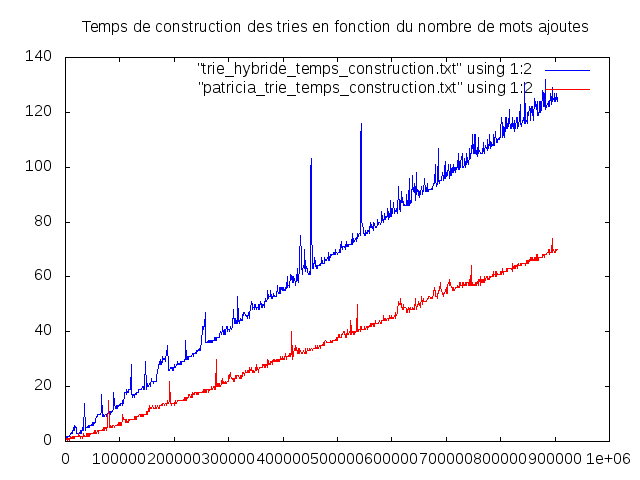
\includegraphics{../comparaison/courbe_temps_construction.png}
\begin{figure}[!htbp]
\caption{Courbe du temps de calcul en fonction du nombre d'ajouts}
\end{figure}

D'après la courbe obtenue, le temps de construction d'un trie hybride et d'un PATRICIA trie semble être en $\Theta$(n).
Ce qui est en adéquation avec l'étude théorique puisque les deux implantations de tries effectuent, pour la construction,
une recherche dans un premier temps et ensuite l'ajout.
La différence observée au niveau de la courbe est vraisemblablement dû en raison du trie hybride qui possède des noeuds-lettre
et le PATRICIA trie des noeuds-chaine-de-caractère.

\section{Temps de suppression}
Le temps de suppression en chargeant dans les tries les œuvres de Shakespeare et en supprimant un ensemble de mot avec un pas
de 1000.\\
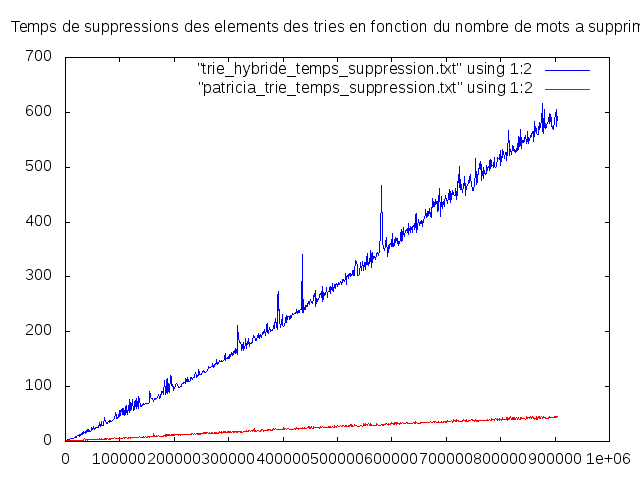
\includegraphics{../comparaison/courbe_temps_suppression.png}
\begin{figure}[!htbp]
\caption{Courbe du temps de calcul en fonction du nombre de suppression}
\end{figure}

D'après la courbe obtenue, le temps de construction d'un trie hybride et d'un PATRICIA trie semble être en $\Theta$(n).
Ce qui est en adéquation avec l'étude théorique puisque les deux implantations de tries effectuent, pour la suppression,
une recherche dans un premier temps, ensuite une suppression et enfin une consolidation de cohérence.
La différence observée au niveau de la courbe est vraisemblablement dû en nombre d'accès de noeuds. En effet, le trie hybride
effectue une recherche plus longue par rapport au PATRICIA trie en raison de leurs structures. De plus, le maintient de la
cohérence des tries oblige encore des parcours dans les fils pour supprimer les noeuds qui ne possèdent pas de mots.

\section{Temps d'ajout d'un mot}
Nous avons aussi calculé le temps d'ajout d'un mot dans des tries qui avaient les œuvres de Shakespeare déjà chargées. Nous avons alors
ajouté des mots français de longueur croissante, dont le plus long mot est composé de 25 lettres.\\
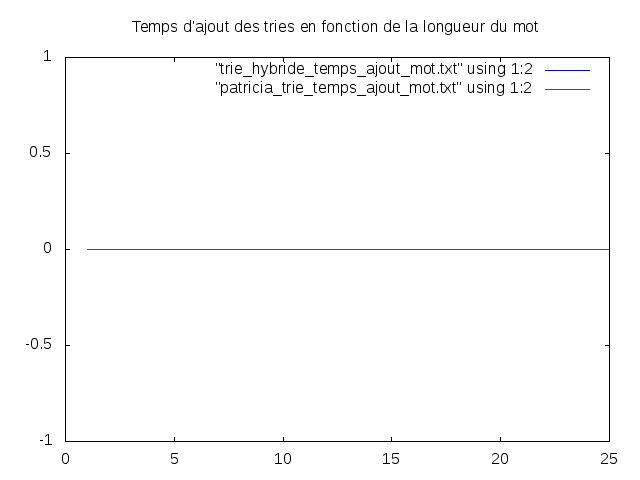
\includegraphics{../comparaison/courbe_ajout_mot.png}
\begin{figure}[!htbp]
\caption{Courbe du temps de calcul en fonction de la longueur du mot}
\end{figure}

Nous pouvons remarquer que le temps d'ajout d'un mot, que cela soit dans un trie hybride ou un PATRICIA trie, est négligeable
puisque la taille d'un mot français ne prend que rarement de grande valeur (en nombre de lettres).

\section{Profondeur moyenne des structures}
Cette étude de la profondeur des structures permet de mettre en évidence l'évolution de la profondeur moyenne des structures
suivant le nombre de mots contenus. Nous avons chargé les œuvres de Shakespeare avec un pas de 1000 et en calculant la profondeur
moyenne entre ces ajouts.\\
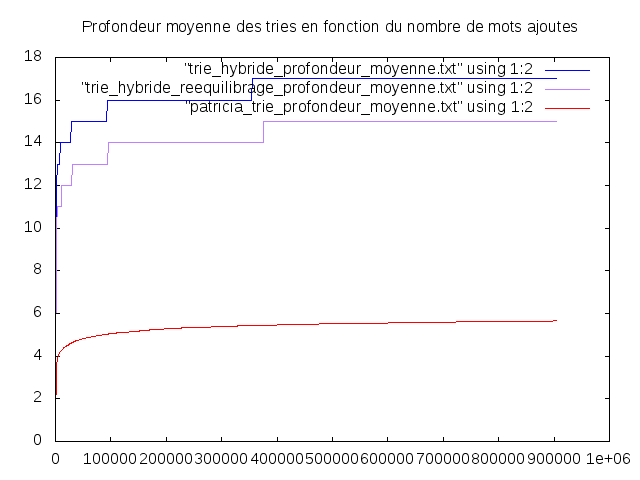
\includegraphics{../comparaison/courbe_profondeur_moyenne.png}
\begin{figure}[!htbp]
\caption{Courbe de la profondeur moyenne en fonction du nombre d'ajouts}
\end{figure}

Au niveau de cette courbe, nous remarquons que la profondeur moyenne du PATRICIA trie est nettement inférieure au trie hybride. Ce
qui est en adéquation avec l'étude théorique puisqu'un PATRICIA trie contient une sous-chaine de lettre correspondant à un
préfixe a l'instar du trie hybride dont chaque noeud correspond à une lettre.
Nous pouvons aussi observer que le rééquilibrage permet de réduire notablement la profondeur moyenne du trie hybride.
\section{Hauteur}
De la même manière que pour le calcul de la profondeur moyenne, nous avons chargé les œuvres et Shakespeare avec un pas de 1000
et en calculant la hauteur entre ces ajouts.\\
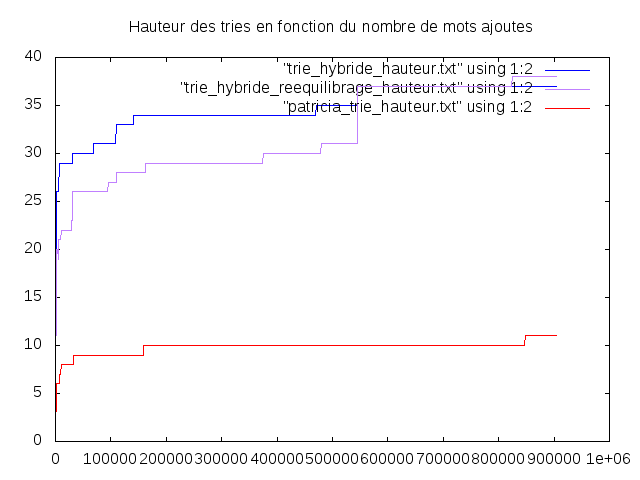
\includegraphics{../comparaison/courbe_hauteur.png}
\begin{figure}[!htbp]
\caption{Courbe de la hauteur en fonction du nombre d'ajouts}
\end{figure}

Au niveau de cette courbe, nous remarquons que la hauteur du PATRICIA trie est nettement inférieure au trie hybride. Ce
qui est en adéquation avec l'étude théorique.
En effet, pour un trie hybride, la hauteur de l'arbre peut être en grande partie dû à la longueur du mot \textit{L} puisqu'un noeud
ne peut contenir qu'une lettre. On a donc toujours une hauteur $\geq$\textit{L} pour un trie hybride alors que pour un PATRICIA trie
la longueur d'un mot peut au mieux être inclus entièrement dans un seul PATRICIA trie.
Nous pouvons aussi observer que le rééquilibrage permet dans certain cas de réduire la hauteur de l'arbre, cependant
il n'est parfois pas possible de réduire en raison de la longueur du mot.

\chapter{Conclusion}
A la suite de cette étude à la fois théorique et expérimentale, nous pouvons conclure que le PATRICIA trie semble l'implantation
la plus efficace en terme de rapidité. Non seulement, le temps de construction est faible comparé au trie hybride, le temps de 
suppression, la profondeur moyenne et la hauteur semble jouer en faveur du PATRICIA trie.
Cependant, il est important de noté l'occupation mémoire de PATRICIA trie, en effet, le PATRICIA trie comporte pour chaque
noeud un tableau de 27 cases afin de stocker ses fils alors que pour le trie hybride il n'en suffit que 3. Dans le cas où 
les mots chargés sont très nombreux et variés, il semblerait que le PATRICIA trie serait plus coûteux en mémoire qu'un trie
hybride.
Ainsi le PATRICIA trie serait plus adéquat pour un dictionnaire de taille moyenne nécessitant des accès rapides alors que le 
trie hybride serait plus utilie pour stocker un dictionnaire de grande taille.


\end{document}
